\section{Practical Instantiation: SSAPO Algorithm}
\label{sec:ssapo}
We now present a \emph{practical} and \emph{computationally tractable} realization of SGPO, 
called \emph{Stackelberg Self-Annotated Preference Optimization (SSAPO)}. 
This method approximates the iterative leader--follower updates 
of Theorem~\ref{thm:convergence_iterative_detailed} 
and Eqs.~\eqref{eq:iterative_update_policy}--\eqref{eq:iterative_update_distribution}, 
overcoming three major challenges in realistic preference alignment:

\begin{compactenum}
    \item \emph{Minimal Human Labels via Self-Annotation.}  We begin with a small “seed” of human-labeled preferences and augment the dataset 
    by letting the \emph{current policy} rank its own responses on unlabeled prompts.
    \item \emph{Convexity/Concavity Mismatch.} When the function $\ell(\cdot)$ is \emph{concave}, the DRO literature \citet{Esfahani2018Data} provides a finite-dimensional $\max$-form program that solves the follower update. However $\ell(\xi) = -\!\log\,\sigma(\xi)$ is convex in $\xi$. We therefore approximate $\ell(\xi)$ by a piecewise-linear \emph{concave} function. 
    \item \emph{Scalability via Uniform Grouping.} 
    For large-scale datasets (potentially hundreds of thousands of preferences), we split the data into subsets and solve each subset’s robust problem in parallel, then merge solutions to form an adversarial $P^*$ for the entire set.
\end{compactenum}

Below, we restate the relevant DRO theorem and describe how to approximate 
$-\!\log\,\sigma(\xi)$ by a concave, piecewise-linear function 
for solving the follower update (Section~\ref{subsec:follower_update}). 
We then detail how SSAPO’s leader--follower loop integrates \emph{self-annotation} and \emph{uniform grouping} (Section~\ref{subsec:ssapo_algorithm}), and finally discuss the impact of these approximations on SGPO’s theoretical guarantees.

\subsection{Solving the Follower's Update with DRO}
\label{subsec:follower_update}
\subsubsection{Construct Worst-Case Distribution}
\label{subsec:concavity_dro_theorem}

Consider the distributionally robust problem
% \begin{equation*}
$$
\label{eq:DRO_concave}
\sup_{P \,\in\, B_\epsilon(\hat{P}_N)}\,\;
\mathbb{E}_P\bigl[\ell(\xi)\bigr], 
% \end{equation*}
$$

$\hat{P}_N = \tfrac1N \sum_{i=1}^N \delta_{\hat{\xi}_i},
B_\epsilon(\hat{P}_N)=\Bigl\{
  P : W(P,\hat{P}_N)\le \epsilon
\Bigr\}.$

\citet{Esfahani2018Data} show that if $\ell(\xi)$ is 
\emph{concave}, then 
$\sup_{P} \mathbb{E}_P[\ell(\xi)]$
admits a \emph{finite convex program} in the variables 
$\{\alpha_{ik}, q_{ik}\}$ whose solution yields 
a worst-case \emph{extremal distribution} $P^*\in B_\epsilon(\hat{P}_N)$.  
Conceptually, each original sample $\hat{\xi}_i$ can “shift” by $q_{ik}/\alpha_{ik}$ 
subject to $\ell(\cdot)$ being evaluated at $\hat{\xi}_i - (q_{ik}/\alpha_{ik})$.  
In the $\max$-form, that shift tries to \emph{increase} 
$\ell(\xi)$ in a worst-case sense. Formally.

\begin{theorem}[Worst-Case Extremal Distributions, specialized from Theorem 4.4 in \citealp{Esfahani2018Data}]
\label{thm:worst_case_concave}
If $\ell(\cdot)$ is proper, concave, and lower semicontinuous on $\Xi \subset \mathbb{R}^m$, 
then
\begin{tiny}
\begin{align*}
\sup_{P\in B_\epsilon(\hat{P}_N)}
\mathbb{E}_P\bigl[\ell(\xi)\bigr]=\max_{\substack{\alpha_{ik},\,q_{ik}\\i=1,\dots,N;\,k=1,\dots,K}}
\frac{1}{N} \sum_{i=1}^N \sum_{k=1}^K
\alpha_{ik}
\,\ell\Bigl(\hat{\xi}_i-\tfrac{q_{ik}}{\alpha_{ik}}\Bigr)
\end{align*}
\end{tiny}
subject to the usual Wasserstein and feasibility constraints
$\tfrac{1}{N}\sum_{i,k}\|q_{ik}\|\le \epsilon$, 
$\sum_{k}\alpha_{ik}=1, \alpha_{ik}\ge 0$, and 
$\hat{\xi}_i-\tfrac{q_{ik}}{\alpha_{ik}}\in \Xi$.  
A discrete distribution 
$\tfrac{1}{N}\sum_{i,k} \alpha_{ik} \delta_{\hat{\xi}_i - \tfrac{q_{ik}}{\alpha_{ik}}}$
achieves the supremum, thus providing $P^*\in B_\epsilon(\hat{P}_N)$.
\end{theorem}

Since $\ell(\xi)=-\!\log\,\sigma(\xi)$ is actually \emph{convex} rather than concave, 
we cannot directly apply Theorem~\ref{thm:worst_case_concave}. 
Hence, Section~\ref{subsec:concave_approx} explains how to construct 
a concave \emph{piecewise-linear} under-approximation 
$\widetilde{\ell}(\cdot)\le -\!\log\,\sigma(\cdot)$, 
enabling us to adopt the same finite convex program framework.

\subsubsection{Concave Piecewise-Linear Approximation}
\label{subsec:concave_approx}

To embed our $\ell(\xi)=-\!\log\,\sigma(\xi)$ into 
Theorem~\ref{thm:worst_case_concave}, we construct a \emph{concave under-approximation} 
$\widetilde{\ell}(\xi)$ represented by $K$ linear pieces:
\begin{equation}
\label{eq:piecewise_concave_ell}
\widetilde{\ell}(\xi)
\;=\;
\max_{1\le k\le K}\;\ell_k(\xi),
\end{equation}

where each $\ell_k(\xi)$is an affine function, and
$\forall\,\xi:\;
\widetilde{\ell}(\xi)
\;\;\le\;\;
-\!\log\,\sigma(\xi)$.
Because the $\ell_k(\cdot)$ are linear and we take a $\max$, 
$\widetilde{\ell}(\cdot)$ is indeed a \emph{concave}, piecewise-linear function.  

One practical construction is to partition an interval of interest into $K$ “knots” 
$\{\xi^{(k)}\}$ and define $\ell_k(\xi)$ as the tangent line \emph{from below} 
(or a chord) such that $\ell_k(\xi^{(k)}) = -\!\log\,\sigma(\xi^{(k)})$ 
but $\ell_k(\xi)\le -\!\log\,\sigma(\xi)$ for all $\xi$ in the domain.  
Equidistant points can be taken in the interval $[0,1]$, considering the image of sigmoid activations $\sigma(\cdot)$ is $[0,1]$.

\paragraph{Follower’s DRO Problem with $\widetilde{\ell}(\cdot)$.}
Replacing $\ell(\xi)$ in Theorem~\ref{thm:worst_case_concave} with 
$\widetilde{\ell}(\xi)$ gives a \emph{finite convex program} that yields 
$P^*\in B_\epsilon(\hat{P}_N)$.  Concretely, 
\begin{small}
  \begin{equation}
\label{eq:widetilde_dro}
\max_{P \in B_\epsilon(\hat{P}_N)}
\mathbb{E}_P[\widetilde{\ell}(\xi)]
=
\max_{\,\{\alpha_{ik},\,q_{ik}\}}
\;\;
\frac{1}{N}
\sum_{i=1}^N
\sum_{k=1}^K
\alpha_{ik}
\;\ell_k\!\Bigl(\hat{\xi}_i \;-\; \tfrac{q_{ik}}{\alpha_{ik}}\Bigr),
\end{equation}  
\end{small}
subject to standard Wasserstein constraints.  
Since $\widetilde{\ell}(\xi)\le -\!\log\,\sigma(\xi)$, 
this \emph{under-approximation} yields a $P^*$ that is valid---but 
\emph{less adversarial}---for the original $\ell(\xi)$.

\subsection{SSAPO: Algorithmic Steps}
\label{subsec:ssapo_algorithm}
\begin{figure}[t]
\centering
\resizebox{0.95\columnwidth}{!}{%
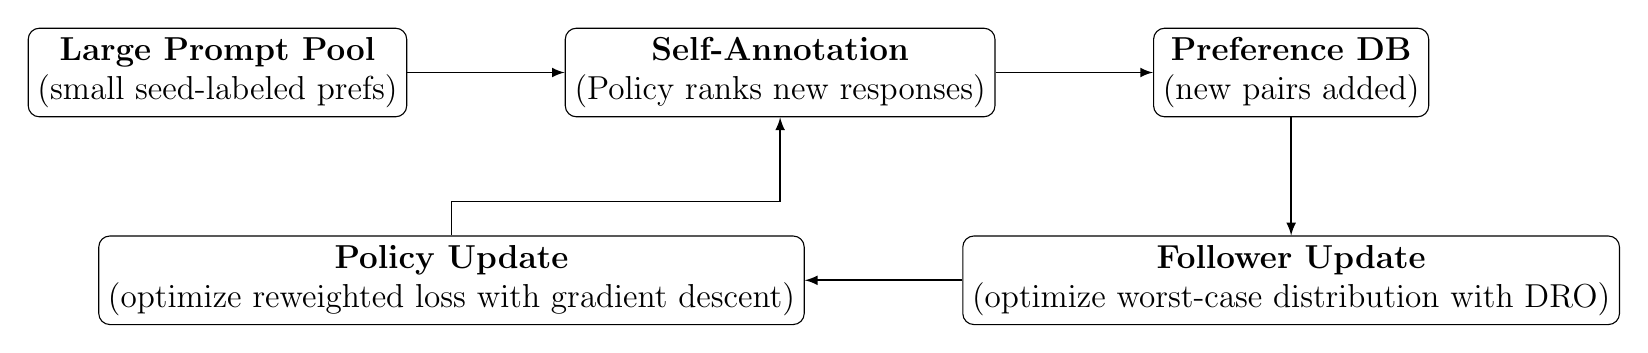
\begin{tikzpicture}[
    font=\large, % <-- Makes text in the nodes larger
    node distance=2.0cm,
    >=latex,
    box/.style={
      rectangle,
      draw=black,
      rounded corners,
      align=center,
      minimum width=2.4cm,
      minimum height=1.1cm
    }
]
\usetikzlibrary{arrows.meta, positioning, calc}

%--- Nodes ---
\node[box] (prompts) {
  \textbf{Large Prompt Pool} \\
  (small seed-labeled prefs)
};
\node[box, right=2.0cm of prompts] (selfanno) {
  \textbf{Self-Annotation} \\
  (Policy ranks new responses)
};
\node[box, right=2.0cm of selfanno] (prefdb) {
  \textbf{Preference DB} \\
  (new pairs added)
};
\node[box, below=1.5cm of prefdb] (dro) {
  \textbf{Follower Update} \\
  (optimize worst-case distribution with DRO)
};
\node[box, left=2.0cm of dro] (policy) {
  \textbf{Policy Update} \\
  (optimize reweighted loss with gradient descent)
};

%--- Arrows ---
\draw[->, line width=0.6pt] (prompts) -- (selfanno);
\draw[->, line width=0.6pt] (selfanno) -- (prefdb);
\draw[->, line width=0.6pt] (prefdb) -- (dro);
\draw[->, line width=0.6pt] (dro) -- (policy);
\draw[->, line width=0.6pt] (policy) -- ++(0,1.0) -| (selfanno);

\end{tikzpicture}%
}
\caption{%
\textbf{SSAPO workflow.} 
We maintain a large prompt pool and a small set of seed-labeled preferences. 
The policy self-annotates new prompts by generating and ranking responses, 
thus expanding the preference database. 
A follower then identifies a worst-case distribution 
for these preferences, 
and the leader (policy) is updated accordingly. 
This process repeats for multiple iterations.
}
\label{fig:ssapo_framework}
\end{figure}

Figure~\ref{fig:ssapo_framework} summarizes the SSAPO workflow. 
Starting with a small seed of human-labeled preferences plus a large unlabeled pool, 
we proceed in the following loop:

\begin{compactenum}
\item \emph{Self-Annotation.}  
  At each iteration, we sample new unlabeled prompts from 
  $\mathcal{D}_{\mathrm{unlabeled}}$ and let the current policy 
  $\pi_{\theta_t}$ generate candidate responses.  The policy \emph{ranks} them 
  to form winner-loser pairs $(y_w,y_l)$, which expand the preference dataset 
  $\mathcal{D}$.  From these, we build $\hat{\xi}_i = R_{\theta_t}(y_w^i) - R_{\theta_t}(y_l^i)$.

\item \emph{Concave Piecewise-Linear Approx.}  
  We fix $K$ and define $\{\ell_k\}_{k=1}^K$ such that 
  $\widetilde{\ell}(\xi) = \max_k \ell_k(\xi)\le -\!\log\,\sigma(\xi)$ 
  (as in Eq.~\eqref{eq:piecewise_concave_ell}).  

\item \emph{Worst-Case Distribution.}  
  We form $\hat{P}_N=\tfrac1N\sum_{i=1}^N \delta_{\hat{\xi}_i}$, 
  then solve Eq.~\eqref{eq:widetilde_dro} with $\widetilde{\ell}$.  
  By Theorem~\ref{thm:worst_case_concave}, the solution is a discrete distribution 
  $P^*_t \in B_\epsilon(\hat{P}_N)$ that \emph{shifts} each $\hat{\xi}_i$ 
  by up to $q_{ik}^{*}/\alpha_{ik}^{*}$, then applies the affine $\ell_k(\cdot)$ 
  and weights $\alpha_{ik}^{*}$.  

\item \emph{Policy Update.}  
  We train $\pi_{\theta}$ on $P^*_t$ by minimizing 
  $\mathbb{E}_{P^*_t}\bigl[-\!\log\,\sigma(R_\theta(y_w)-R_\theta(y_l))\bigr]$.  
  Noting that $P^*_t$ identifies how often each shifted $\xi_i$ is “activated,” 
  we can equivalently reweight the original samples for gradient-based updates.
\end{compactenum}

Repeating for $T$ total iterations yields the final aligned policy $\pi_{\theta_T}$. A more explicit version of SSAPO is provided in Algorithm~\ref{algo:ssapo} (Appendix~\ref{sec:SSAPO_algorithm+analysis}), along with its computational complexity analysis.

\subsubsection{Scalability via Uniform Grouping and Approximation}
\label{subsec:discussion_approx}

\paragraph{Grouping Large Datasets.}
When $N$ is large (e.g.\ $\!10^5\!$ or more preferences), solving the convex program 
in Step~(Worst-Case Distribution) can be expensive.  A popular heuristic partitions 
$\{\hat{\xi}_1,\dots,\hat{\xi}_N\}$ into $M$ groups (each of size $G=N/M$), 
and solves the finite program \eqref{eq:widetilde_dro} separately within each group.   %One may resort to primal-dual or specialized cutting-plane
%methods \citep{Esfahani2018DataDrivenDR}, or use approximate relaxations with 
%entropic regularization \citep{Cuturi2013Sinkhorn}.
The resulting distributions $P^*_m$ are then averaged (or merged proportionally):
$$
P_{\mathrm{final}}^*
\;=\;
\frac{1}{M}
\sum_{m=1}^M
P^*_m.
$$
While not an \emph{exact} solution to the global $N$-sample problem, 
this still confers substantial robustness while reducing complexity from 
$N$ to $G \ll N$ in each subproblem. In summary, this grouping approach greatly reduces memory/compute cost, and is parallelizable.
%Alternatives include \emph{mini-batch} sampling \citep{Blanchet2019quantifying} 
%and \emph{clustering} \citep{Khezeli2019,Gao2022distributionally}.

\begin{remark}[Approximation Effects on SGPO Guarantees]
    Two approximations separate SSAPO from the ideal solution of 
Section~\ref{sec:theory}: (1) \emph{Concave Under-Approximation:}  
 Replacing $-\!\log\,\sigma(\cdot)$ with its piecewise-linear approximation $\widetilde{\ell}(\cdot)$ (i.e., $\widetilde{\ell}(\xi)\le -\!\log\,\sigma(\xi)$) ensures feasibility in Theorem~\ref{thm:worst_case_concave}, but slightly weakens the adversarial effect. Consequently, the policy may be \emph{less robust} than in the fully ideal solution $\max_{P}\!\mathbb{E}_P[-\!\log\,\sigma(\cdot)]$. Increasing $K$ (i.e., refining the linear approximation) narrows this gap. (2)\emph{Partitioned Solver:}   Rather than solving one global $\arg\max_{P \in B_\epsilon(\hat{P}_N)}$, SSAPO partitions the dataset into $M$ groups and separately solves $M$ subproblems. Merging their solutions may deviate from a unified optimum, but it still explores adversarial reweighting in each subgroup, preserving much of SGPO’s robustness against distributional shifts.
\end{remark}

\vspace{-0.1 in}
Despite these approximations, SSAPO preserves the \emph{Stackelberg} essence: the policy is trained against worst-case reweightings within an $\epsilon$-Wasserstein distance. As a result, it retains the key benefit of \emph{bounded regret} for moderate shifts (Theorem~\ref{thm:sgpo_regret}), while remaining computationally tractable. Indeed, if $K \!\to\! \infty$ and $M\!=\!1$, SSAPO recovers the exact follower solution (subject to sampling). Empirically (Section~\ref{sec:experiments}), these approximations still yield substantial label-efficiency and robustness gains over standard DPO.

%\paragraph{Effects on SGPO Guarantees.}
%\begin{enumerate}
%    \item \textbf{Concave Under-Approximation:}  
%      Using $\widetilde{\ell}(\xi)\le -\!\log\,\sigma(\xi)$ ensures feasibility 
%      in Theorem~\ref{thm:worst_case_concave}, but reduces the adversary’s effect.  
%      Hence, the policy may be slightly \emph{less robust} than the ideal solution 
%      of $\max_{P}\mathbb{E}_P[-\!\log\,\sigma(\cdot)]$.  Increasing $K$ 
%      (refining the linear segments) narrows this gap.
%   \item \textbf{Partitioned Solver:}  
%      Instead of one global $\arg\max_{P\in B_\epsilon(\hat{P}_N)}$, 
%      grouping effectively solves $M$ separate subproblems and combines them.  
%      This may deviate from a single unified optimum distribution.  
%      Nonetheless, each partial subproblem still explores adversarial 
%      reweighting, retaining a significant portion of SGPO’s protection 
%      against distributional shifts.
%\end{enumerate}

%Despite these approximations, SSAPO retains the essential \emph{Stackelberg} nature:
%the policy trains against a worst-case reweighting of preferences within 
%\(\epsilon\)-Wasserstein distance.  Consequently, SSAPO still reaps the main %benefits 
%of bounded regret under moderate shifts (Theorem~\ref{thm:sgpo_regret}),
%while ensuring practical feasibility.
%As $K\to\infty$ and $M=1$ (no partitioning), SSAPO recovers the full 
%follower’s solution (subject to the sample-based approximation).  
%In practice, these approximations offer a favorable balance between 
%robustness and computational feasibility.
%Empirical results in Section~\ref{sec:experiments}
%demonstrate label-efficiency and robustness gains relative to standard DPO.